\documentclass[10pt]{beamer}

  % Math Packages
  \usepackage{amsmath}
  \usepackage{amsthm}
  \usepackage{mathtools}

  % Graphics Packages
  \usepackage{graphicx}
  \usepackage{pgf}
  \usepackage[export]{adjustbox}

  % Colors
  \definecolor{umared}{RGB}{255,74,74}
  \definecolor{mygray}{RGB}{66,66,66}

  % Theme Settings
  \usetheme{metropolis}

  \setbeamercolor{normal text}{fg=mygray}
  \setbeamercolor{alerted text}{fg=umared}
  \setbeamercolor{title text}{fg=mygray}
  \setbeamercolor{title separator}{fg=umared}
  \setbeamercolor{progress bar}{fg=umared}
  \setbeamercolor{frametitle}{bg=umared}

\title{Oracle Taxation Theory}
\logo{
  \makebox[0.13\paperwidth]{\includegraphics[width=1.5cm,keepaspectratio]{Uma_Logo.png} \hfill}
}
\date[]{\today}

\begin{document}

% Title Slide
\begin{frame}
  \titlepage
\end{frame}

% --------------------------------------- %
% Introduction
% --------------------------------------- %
\section{Introduction}

\begin{frame} \frametitle{What do we want to accomplish}

  Questions we are interested in:

  \begin{itemize}
    \item System security\textemdash{Cost of Corruption > Profit from Corruption}
    \item Understand effect tax rate in relation to equilibrium token price
    \item Dynamic tax rates to induce secure token price \alert{(Not Today)}
  \end{itemize}

\end{frame}

\begin{frame} \frametitle{Goals}

  Why economic theory?

  \begin{itemize}
    \item Safe environment for ``testing''
    \item Mathematical formalism makes assumptions transparent
    \item Often learn new things about the environment we build
  \end{itemize}

\end{frame}

% --------------------------------------- %
% Model
% --------------------------------------- %
\section{Model Structure}

\begin{frame} \frametitle{Overview}

  \begin{center}
    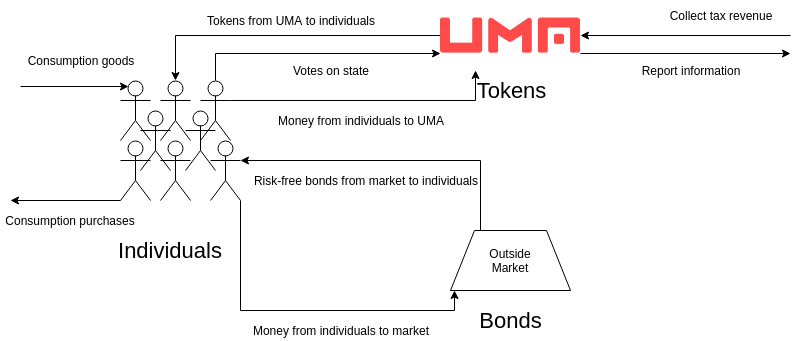
\includegraphics[width=0.8\paperwidth]{ModelOverview.png}
  \end{center}

\end{frame}

\begin{frame} \frametitle{Details: Oracle}

  Must report information to derivatives market, but cannot verify the
  information on its own

  Requires others to vote on information

  Oracle sells voting rights and raises tax revenue ($\mu$ margin taxed at $\tau$)

  Uses revenue to incentivize people to reveal the needed information

\end{frame}

\begin{frame} \frametitle{Details: Individuals}

  There are many individuals

  Each individual likes to eat consumption goods

  Can save for tomorrow using bonds or tokens

\end{frame}

\begin{frame} \frametitle{Details: Voting}

  If an individual owns tokens, they vote on information Oracle must report

  If they choose to tell the truth then

  \begin{itemize}
    \item With probability $\eta$, they forget to vote
    \item With probability $\pi$, they make a mistake
  \end{itemize}

  Liars are deliberate... No forgetting and no mistakes

  Equilibrium concept is \textit{Perfect Bayesian Equilibrium} \textemdash{
  Everyone believes that everyone else will attempt to tell truth}

\end{frame}

\begin{frame} \frametitle{Details: Wealth Evolution}

  If you, and everyone else, attempt to tell truth then

  \begin{align*}
    w_{t+1} &= \begin{cases} (1 + r) b + q x \quad \text{if forget} \\
                             (1 + r) b + (1 + \gamma \frac{\pi}{1 - \pi}) (q + \mu \tau) x \quad \text{if report truth} \\
                             (1 + r) b + (1 - \gamma) (q + \mu \tau) x \quad \text{if mistake} \\
               \end{cases}
  \end{align*}

  If you lie then

  \begin{align*}
    w_{t+1} &= \begin{cases} (1 + r)b + (1 + \gamma \frac{1 - \pi}{\pi})(\mu \tau + {\color{red} 0}) x + {\color{red}\kappa \mu} \quad \text{if corrupted} \\
                             (1 + r)b + (1 - \gamma)(\mu \tau + q) x \quad \text{if not corrupted}
               \end{cases}
  \end{align*}

\end{frame}

% --------------------------------------- %
% Results
% --------------------------------------- %
\section{Results}

\begin{frame} \frametitle{Risk-Neutral Pricing}

  If there all individuals were risk-neutral investors, then the token market
  cap would be its expected discounted returns

  \begin{align*}
    q = E \left[ \sum_{t=0}^{\infty} \left(\frac{1}{1 + r} \right)^t (\text{dividend payment}) \right]
  \end{align*}

\end{frame}

\begin{frame} \frametitle{Risk-Neutral Pricing}

  With 1,000,000 in margin and a (yearly) discount rate of $r = 0.04$

  \begin{center}
    \resizebox{0.8\textwidth}{!}{%% Creator: Matplotlib, PGF backend
%%
%% To include the figure in your LaTeX document, write
%%   \input{<filename>.pgf}
%%
%% Make sure the required packages are loaded in your preamble
%%   \usepackage{pgf}
%%
%% Figures using additional raster images can only be included by \input if
%% they are in the same directory as the main LaTeX file. For loading figures
%% from other directories you can use the `import` package
%%   \usepackage{import}
%% and then include the figures with
%%   \import{<path to file>}{<filename>.pgf}
%%
%% Matplotlib used the following preamble
%%   \usepackage{fontspec}
%%   \setmainfont{DejaVu Serif}
%%   \setsansfont{DejaVu Sans}
%%   \setmonofont{DejaVu Sans Mono}
%%
\begingroup%
\makeatletter%
\begin{pgfpicture}%
\pgfpathrectangle{\pgfpointorigin}{\pgfqpoint{6.400000in}{4.800000in}}%
\pgfusepath{use as bounding box, clip}%
\begin{pgfscope}%
\pgfsetbuttcap%
\pgfsetmiterjoin%
\pgfsetlinewidth{0.000000pt}%
\definecolor{currentstroke}{rgb}{0.000000,0.000000,0.000000}%
\pgfsetstrokecolor{currentstroke}%
\pgfsetstrokeopacity{0.000000}%
\pgfsetdash{}{0pt}%
\pgfpathmoveto{\pgfqpoint{0.000000in}{0.000000in}}%
\pgfpathlineto{\pgfqpoint{6.400000in}{0.000000in}}%
\pgfpathlineto{\pgfqpoint{6.400000in}{4.800000in}}%
\pgfpathlineto{\pgfqpoint{0.000000in}{4.800000in}}%
\pgfpathclose%
\pgfusepath{}%
\end{pgfscope}%
\begin{pgfscope}%
\pgfsetbuttcap%
\pgfsetmiterjoin%
\pgfsetlinewidth{0.000000pt}%
\definecolor{currentstroke}{rgb}{0.000000,0.000000,0.000000}%
\pgfsetstrokecolor{currentstroke}%
\pgfsetstrokeopacity{0.000000}%
\pgfsetdash{}{0pt}%
\pgfpathmoveto{\pgfqpoint{0.800000in}{0.528000in}}%
\pgfpathlineto{\pgfqpoint{5.760000in}{0.528000in}}%
\pgfpathlineto{\pgfqpoint{5.760000in}{4.224000in}}%
\pgfpathlineto{\pgfqpoint{0.800000in}{4.224000in}}%
\pgfpathclose%
\pgfusepath{}%
\end{pgfscope}%
\begin{pgfscope}%
\pgfsetbuttcap%
\pgfsetroundjoin%
\definecolor{currentfill}{rgb}{0.000000,0.000000,0.000000}%
\pgfsetfillcolor{currentfill}%
\pgfsetlinewidth{0.803000pt}%
\definecolor{currentstroke}{rgb}{0.000000,0.000000,0.000000}%
\pgfsetstrokecolor{currentstroke}%
\pgfsetdash{}{0pt}%
\pgfsys@defobject{currentmarker}{\pgfqpoint{0.000000in}{-0.048611in}}{\pgfqpoint{0.000000in}{0.000000in}}{%
\pgfpathmoveto{\pgfqpoint{0.000000in}{0.000000in}}%
\pgfpathlineto{\pgfqpoint{0.000000in}{-0.048611in}}%
\pgfusepath{stroke,fill}%
}%
\begin{pgfscope}%
\pgfsys@transformshift{1.025455in}{0.528000in}%
\pgfsys@useobject{currentmarker}{}%
\end{pgfscope}%
\end{pgfscope}%
\begin{pgfscope}%
\pgftext[x=1.025455in,y=0.430778in,,top]{\sffamily\fontsize{10.000000}{12.000000}\selectfont 0}%
\end{pgfscope}%
\begin{pgfscope}%
\pgfsetbuttcap%
\pgfsetroundjoin%
\definecolor{currentfill}{rgb}{0.000000,0.000000,0.000000}%
\pgfsetfillcolor{currentfill}%
\pgfsetlinewidth{0.803000pt}%
\definecolor{currentstroke}{rgb}{0.000000,0.000000,0.000000}%
\pgfsetstrokecolor{currentstroke}%
\pgfsetdash{}{0pt}%
\pgfsys@defobject{currentmarker}{\pgfqpoint{0.000000in}{-0.048611in}}{\pgfqpoint{0.000000in}{0.000000in}}{%
\pgfpathmoveto{\pgfqpoint{0.000000in}{0.000000in}}%
\pgfpathlineto{\pgfqpoint{0.000000in}{-0.048611in}}%
\pgfusepath{stroke,fill}%
}%
\begin{pgfscope}%
\pgfsys@transformshift{1.626744in}{0.528000in}%
\pgfsys@useobject{currentmarker}{}%
\end{pgfscope}%
\end{pgfscope}%
\begin{pgfscope}%
\pgftext[x=1.626744in,y=0.430778in,,top]{\sffamily\fontsize{10.000000}{12.000000}\selectfont 20}%
\end{pgfscope}%
\begin{pgfscope}%
\pgfsetbuttcap%
\pgfsetroundjoin%
\definecolor{currentfill}{rgb}{0.000000,0.000000,0.000000}%
\pgfsetfillcolor{currentfill}%
\pgfsetlinewidth{0.803000pt}%
\definecolor{currentstroke}{rgb}{0.000000,0.000000,0.000000}%
\pgfsetstrokecolor{currentstroke}%
\pgfsetdash{}{0pt}%
\pgfsys@defobject{currentmarker}{\pgfqpoint{0.000000in}{-0.048611in}}{\pgfqpoint{0.000000in}{0.000000in}}{%
\pgfpathmoveto{\pgfqpoint{0.000000in}{0.000000in}}%
\pgfpathlineto{\pgfqpoint{0.000000in}{-0.048611in}}%
\pgfusepath{stroke,fill}%
}%
\begin{pgfscope}%
\pgfsys@transformshift{2.228033in}{0.528000in}%
\pgfsys@useobject{currentmarker}{}%
\end{pgfscope}%
\end{pgfscope}%
\begin{pgfscope}%
\pgftext[x=2.228033in,y=0.430778in,,top]{\sffamily\fontsize{10.000000}{12.000000}\selectfont 40}%
\end{pgfscope}%
\begin{pgfscope}%
\pgfsetbuttcap%
\pgfsetroundjoin%
\definecolor{currentfill}{rgb}{0.000000,0.000000,0.000000}%
\pgfsetfillcolor{currentfill}%
\pgfsetlinewidth{0.803000pt}%
\definecolor{currentstroke}{rgb}{0.000000,0.000000,0.000000}%
\pgfsetstrokecolor{currentstroke}%
\pgfsetdash{}{0pt}%
\pgfsys@defobject{currentmarker}{\pgfqpoint{0.000000in}{-0.048611in}}{\pgfqpoint{0.000000in}{0.000000in}}{%
\pgfpathmoveto{\pgfqpoint{0.000000in}{0.000000in}}%
\pgfpathlineto{\pgfqpoint{0.000000in}{-0.048611in}}%
\pgfusepath{stroke,fill}%
}%
\begin{pgfscope}%
\pgfsys@transformshift{2.829322in}{0.528000in}%
\pgfsys@useobject{currentmarker}{}%
\end{pgfscope}%
\end{pgfscope}%
\begin{pgfscope}%
\pgftext[x=2.829322in,y=0.430778in,,top]{\sffamily\fontsize{10.000000}{12.000000}\selectfont 60}%
\end{pgfscope}%
\begin{pgfscope}%
\pgfsetbuttcap%
\pgfsetroundjoin%
\definecolor{currentfill}{rgb}{0.000000,0.000000,0.000000}%
\pgfsetfillcolor{currentfill}%
\pgfsetlinewidth{0.803000pt}%
\definecolor{currentstroke}{rgb}{0.000000,0.000000,0.000000}%
\pgfsetstrokecolor{currentstroke}%
\pgfsetdash{}{0pt}%
\pgfsys@defobject{currentmarker}{\pgfqpoint{0.000000in}{-0.048611in}}{\pgfqpoint{0.000000in}{0.000000in}}{%
\pgfpathmoveto{\pgfqpoint{0.000000in}{0.000000in}}%
\pgfpathlineto{\pgfqpoint{0.000000in}{-0.048611in}}%
\pgfusepath{stroke,fill}%
}%
\begin{pgfscope}%
\pgfsys@transformshift{3.430611in}{0.528000in}%
\pgfsys@useobject{currentmarker}{}%
\end{pgfscope}%
\end{pgfscope}%
\begin{pgfscope}%
\pgftext[x=3.430611in,y=0.430778in,,top]{\sffamily\fontsize{10.000000}{12.000000}\selectfont 80}%
\end{pgfscope}%
\begin{pgfscope}%
\pgfsetbuttcap%
\pgfsetroundjoin%
\definecolor{currentfill}{rgb}{0.000000,0.000000,0.000000}%
\pgfsetfillcolor{currentfill}%
\pgfsetlinewidth{0.803000pt}%
\definecolor{currentstroke}{rgb}{0.000000,0.000000,0.000000}%
\pgfsetstrokecolor{currentstroke}%
\pgfsetdash{}{0pt}%
\pgfsys@defobject{currentmarker}{\pgfqpoint{0.000000in}{-0.048611in}}{\pgfqpoint{0.000000in}{0.000000in}}{%
\pgfpathmoveto{\pgfqpoint{0.000000in}{0.000000in}}%
\pgfpathlineto{\pgfqpoint{0.000000in}{-0.048611in}}%
\pgfusepath{stroke,fill}%
}%
\begin{pgfscope}%
\pgfsys@transformshift{4.031901in}{0.528000in}%
\pgfsys@useobject{currentmarker}{}%
\end{pgfscope}%
\end{pgfscope}%
\begin{pgfscope}%
\pgftext[x=4.031901in,y=0.430778in,,top]{\sffamily\fontsize{10.000000}{12.000000}\selectfont 100}%
\end{pgfscope}%
\begin{pgfscope}%
\pgfsetbuttcap%
\pgfsetroundjoin%
\definecolor{currentfill}{rgb}{0.000000,0.000000,0.000000}%
\pgfsetfillcolor{currentfill}%
\pgfsetlinewidth{0.803000pt}%
\definecolor{currentstroke}{rgb}{0.000000,0.000000,0.000000}%
\pgfsetstrokecolor{currentstroke}%
\pgfsetdash{}{0pt}%
\pgfsys@defobject{currentmarker}{\pgfqpoint{0.000000in}{-0.048611in}}{\pgfqpoint{0.000000in}{0.000000in}}{%
\pgfpathmoveto{\pgfqpoint{0.000000in}{0.000000in}}%
\pgfpathlineto{\pgfqpoint{0.000000in}{-0.048611in}}%
\pgfusepath{stroke,fill}%
}%
\begin{pgfscope}%
\pgfsys@transformshift{4.633190in}{0.528000in}%
\pgfsys@useobject{currentmarker}{}%
\end{pgfscope}%
\end{pgfscope}%
\begin{pgfscope}%
\pgftext[x=4.633190in,y=0.430778in,,top]{\sffamily\fontsize{10.000000}{12.000000}\selectfont 120}%
\end{pgfscope}%
\begin{pgfscope}%
\pgfsetbuttcap%
\pgfsetroundjoin%
\definecolor{currentfill}{rgb}{0.000000,0.000000,0.000000}%
\pgfsetfillcolor{currentfill}%
\pgfsetlinewidth{0.803000pt}%
\definecolor{currentstroke}{rgb}{0.000000,0.000000,0.000000}%
\pgfsetstrokecolor{currentstroke}%
\pgfsetdash{}{0pt}%
\pgfsys@defobject{currentmarker}{\pgfqpoint{0.000000in}{-0.048611in}}{\pgfqpoint{0.000000in}{0.000000in}}{%
\pgfpathmoveto{\pgfqpoint{0.000000in}{0.000000in}}%
\pgfpathlineto{\pgfqpoint{0.000000in}{-0.048611in}}%
\pgfusepath{stroke,fill}%
}%
\begin{pgfscope}%
\pgfsys@transformshift{5.234479in}{0.528000in}%
\pgfsys@useobject{currentmarker}{}%
\end{pgfscope}%
\end{pgfscope}%
\begin{pgfscope}%
\pgftext[x=5.234479in,y=0.430778in,,top]{\sffamily\fontsize{10.000000}{12.000000}\selectfont 140}%
\end{pgfscope}%
\begin{pgfscope}%
\pgftext[x=3.280000in,y=0.240809in,,top]{\sffamily\fontsize{10.000000}{12.000000}\selectfont Years of Dividends}%
\end{pgfscope}%
\begin{pgfscope}%
\pgfsetbuttcap%
\pgfsetroundjoin%
\definecolor{currentfill}{rgb}{0.000000,0.000000,0.000000}%
\pgfsetfillcolor{currentfill}%
\pgfsetlinewidth{0.803000pt}%
\definecolor{currentstroke}{rgb}{0.000000,0.000000,0.000000}%
\pgfsetstrokecolor{currentstroke}%
\pgfsetdash{}{0pt}%
\pgfsys@defobject{currentmarker}{\pgfqpoint{-0.048611in}{0.000000in}}{\pgfqpoint{0.000000in}{0.000000in}}{%
\pgfpathmoveto{\pgfqpoint{0.000000in}{0.000000in}}%
\pgfpathlineto{\pgfqpoint{-0.048611in}{0.000000in}}%
\pgfusepath{stroke,fill}%
}%
\begin{pgfscope}%
\pgfsys@transformshift{0.800000in}{0.695747in}%
\pgfsys@useobject{currentmarker}{}%
\end{pgfscope}%
\end{pgfscope}%
\begin{pgfscope}%
\pgftext[x=0.614413in,y=0.642986in,left,base]{\sffamily\fontsize{10.000000}{12.000000}\selectfont 0}%
\end{pgfscope}%
\begin{pgfscope}%
\pgfsetbuttcap%
\pgfsetroundjoin%
\definecolor{currentfill}{rgb}{0.000000,0.000000,0.000000}%
\pgfsetfillcolor{currentfill}%
\pgfsetlinewidth{0.803000pt}%
\definecolor{currentstroke}{rgb}{0.000000,0.000000,0.000000}%
\pgfsetstrokecolor{currentstroke}%
\pgfsetdash{}{0pt}%
\pgfsys@defobject{currentmarker}{\pgfqpoint{-0.048611in}{0.000000in}}{\pgfqpoint{0.000000in}{0.000000in}}{%
\pgfpathmoveto{\pgfqpoint{0.000000in}{0.000000in}}%
\pgfpathlineto{\pgfqpoint{-0.048611in}{0.000000in}}%
\pgfusepath{stroke,fill}%
}%
\begin{pgfscope}%
\pgfsys@transformshift{0.800000in}{1.369238in}%
\pgfsys@useobject{currentmarker}{}%
\end{pgfscope}%
\end{pgfscope}%
\begin{pgfscope}%
\pgftext[x=0.172586in,y=1.316477in,left,base]{\sffamily\fontsize{10.000000}{12.000000}\selectfont 200000}%
\end{pgfscope}%
\begin{pgfscope}%
\pgfsetbuttcap%
\pgfsetroundjoin%
\definecolor{currentfill}{rgb}{0.000000,0.000000,0.000000}%
\pgfsetfillcolor{currentfill}%
\pgfsetlinewidth{0.803000pt}%
\definecolor{currentstroke}{rgb}{0.000000,0.000000,0.000000}%
\pgfsetstrokecolor{currentstroke}%
\pgfsetdash{}{0pt}%
\pgfsys@defobject{currentmarker}{\pgfqpoint{-0.048611in}{0.000000in}}{\pgfqpoint{0.000000in}{0.000000in}}{%
\pgfpathmoveto{\pgfqpoint{0.000000in}{0.000000in}}%
\pgfpathlineto{\pgfqpoint{-0.048611in}{0.000000in}}%
\pgfusepath{stroke,fill}%
}%
\begin{pgfscope}%
\pgfsys@transformshift{0.800000in}{2.042729in}%
\pgfsys@useobject{currentmarker}{}%
\end{pgfscope}%
\end{pgfscope}%
\begin{pgfscope}%
\pgftext[x=0.172586in,y=1.989968in,left,base]{\sffamily\fontsize{10.000000}{12.000000}\selectfont 400000}%
\end{pgfscope}%
\begin{pgfscope}%
\pgfsetbuttcap%
\pgfsetroundjoin%
\definecolor{currentfill}{rgb}{0.000000,0.000000,0.000000}%
\pgfsetfillcolor{currentfill}%
\pgfsetlinewidth{0.803000pt}%
\definecolor{currentstroke}{rgb}{0.000000,0.000000,0.000000}%
\pgfsetstrokecolor{currentstroke}%
\pgfsetdash{}{0pt}%
\pgfsys@defobject{currentmarker}{\pgfqpoint{-0.048611in}{0.000000in}}{\pgfqpoint{0.000000in}{0.000000in}}{%
\pgfpathmoveto{\pgfqpoint{0.000000in}{0.000000in}}%
\pgfpathlineto{\pgfqpoint{-0.048611in}{0.000000in}}%
\pgfusepath{stroke,fill}%
}%
\begin{pgfscope}%
\pgfsys@transformshift{0.800000in}{2.716220in}%
\pgfsys@useobject{currentmarker}{}%
\end{pgfscope}%
\end{pgfscope}%
\begin{pgfscope}%
\pgftext[x=0.172586in,y=2.663459in,left,base]{\sffamily\fontsize{10.000000}{12.000000}\selectfont 600000}%
\end{pgfscope}%
\begin{pgfscope}%
\pgfsetbuttcap%
\pgfsetroundjoin%
\definecolor{currentfill}{rgb}{0.000000,0.000000,0.000000}%
\pgfsetfillcolor{currentfill}%
\pgfsetlinewidth{0.803000pt}%
\definecolor{currentstroke}{rgb}{0.000000,0.000000,0.000000}%
\pgfsetstrokecolor{currentstroke}%
\pgfsetdash{}{0pt}%
\pgfsys@defobject{currentmarker}{\pgfqpoint{-0.048611in}{0.000000in}}{\pgfqpoint{0.000000in}{0.000000in}}{%
\pgfpathmoveto{\pgfqpoint{0.000000in}{0.000000in}}%
\pgfpathlineto{\pgfqpoint{-0.048611in}{0.000000in}}%
\pgfusepath{stroke,fill}%
}%
\begin{pgfscope}%
\pgfsys@transformshift{0.800000in}{3.389711in}%
\pgfsys@useobject{currentmarker}{}%
\end{pgfscope}%
\end{pgfscope}%
\begin{pgfscope}%
\pgftext[x=0.172586in,y=3.336950in,left,base]{\sffamily\fontsize{10.000000}{12.000000}\selectfont 800000}%
\end{pgfscope}%
\begin{pgfscope}%
\pgfsetbuttcap%
\pgfsetroundjoin%
\definecolor{currentfill}{rgb}{0.000000,0.000000,0.000000}%
\pgfsetfillcolor{currentfill}%
\pgfsetlinewidth{0.803000pt}%
\definecolor{currentstroke}{rgb}{0.000000,0.000000,0.000000}%
\pgfsetstrokecolor{currentstroke}%
\pgfsetdash{}{0pt}%
\pgfsys@defobject{currentmarker}{\pgfqpoint{-0.048611in}{0.000000in}}{\pgfqpoint{0.000000in}{0.000000in}}{%
\pgfpathmoveto{\pgfqpoint{0.000000in}{0.000000in}}%
\pgfpathlineto{\pgfqpoint{-0.048611in}{0.000000in}}%
\pgfusepath{stroke,fill}%
}%
\begin{pgfscope}%
\pgfsys@transformshift{0.800000in}{4.063202in}%
\pgfsys@useobject{currentmarker}{}%
\end{pgfscope}%
\end{pgfscope}%
\begin{pgfscope}%
\pgftext[x=0.084220in,y=4.010440in,left,base]{\sffamily\fontsize{10.000000}{12.000000}\selectfont 1000000}%
\end{pgfscope}%
\begin{pgfscope}%
\pgfpathrectangle{\pgfqpoint{0.800000in}{0.528000in}}{\pgfqpoint{4.960000in}{3.696000in}}%
\pgfusepath{clip}%
\pgfsetbuttcap%
\pgfsetroundjoin%
\pgfsetlinewidth{1.505625pt}%
\definecolor{currentstroke}{rgb}{0.000000,0.000000,0.000000}%
\pgfsetstrokecolor{currentstroke}%
\pgfsetdash{{5.550000pt}{2.400000pt}}{0.000000pt}%
\pgfpathmoveto{\pgfqpoint{1.025455in}{2.379475in}}%
\pgfpathlineto{\pgfqpoint{5.234479in}{2.379475in}}%
\pgfusepath{stroke}%
\end{pgfscope}%
\begin{pgfscope}%
\pgfpathrectangle{\pgfqpoint{0.800000in}{0.528000in}}{\pgfqpoint{4.960000in}{3.696000in}}%
\pgfusepath{clip}%
\pgfsetrectcap%
\pgfsetroundjoin%
\pgfsetlinewidth{1.505625pt}%
\definecolor{currentstroke}{rgb}{1.000000,0.290196,0.290196}%
\pgfsetstrokecolor{currentstroke}%
\pgfsetdash{}{0pt}%
\pgfpathmoveto{\pgfqpoint{1.025455in}{0.698273in}}%
\pgfpathlineto{\pgfqpoint{1.065348in}{0.867947in}}%
\pgfpathlineto{\pgfqpoint{1.108132in}{1.040513in}}%
\pgfpathlineto{\pgfqpoint{1.141665in}{1.169353in}}%
\pgfpathlineto{\pgfqpoint{1.187918in}{1.338175in}}%
\pgfpathlineto{\pgfqpoint{1.237640in}{1.508615in}}%
\pgfpathlineto{\pgfqpoint{1.278690in}{1.641074in}}%
\pgfpathlineto{\pgfqpoint{1.322052in}{1.773851in}}%
\pgfpathlineto{\pgfqpoint{1.365992in}{1.900591in}}%
\pgfpathlineto{\pgfqpoint{1.402995in}{2.002175in}}%
\pgfpathlineto{\pgfqpoint{1.446357in}{2.115104in}}%
\pgfpathlineto{\pgfqpoint{1.503017in}{2.253276in}}%
\pgfpathlineto{\pgfqpoint{1.550426in}{2.361515in}}%
\pgfpathlineto{\pgfqpoint{1.600148in}{2.467929in}}%
\pgfpathlineto{\pgfqpoint{1.646401in}{2.560958in}}%
\pgfpathlineto{\pgfqpoint{1.693811in}{2.650713in}}%
\pgfpathlineto{\pgfqpoint{1.745845in}{2.742985in}}%
\pgfpathlineto{\pgfqpoint{1.789207in}{2.815370in}}%
\pgfpathlineto{\pgfqpoint{1.833726in}{2.885634in}}%
\pgfpathlineto{\pgfqpoint{1.877666in}{2.950967in}}%
\pgfpathlineto{\pgfqpoint{1.920450in}{3.011030in}}%
\pgfpathlineto{\pgfqpoint{1.971907in}{3.079128in}}%
\pgfpathlineto{\pgfqpoint{2.011222in}{3.128106in}}%
\pgfpathlineto{\pgfqpoint{2.063835in}{3.189847in}}%
\pgfpathlineto{\pgfqpoint{2.114135in}{3.245127in}}%
\pgfpathlineto{\pgfqpoint{2.170795in}{3.303163in}}%
\pgfpathlineto{\pgfqpoint{2.226298in}{3.356071in}}%
\pgfpathlineto{\pgfqpoint{2.274864in}{3.399292in}}%
\pgfpathlineto{\pgfqpoint{2.319383in}{3.436655in}}%
\pgfpathlineto{\pgfqpoint{2.365058in}{3.472780in}}%
\pgfpathlineto{\pgfqpoint{2.422874in}{3.515636in}}%
\pgfpathlineto{\pgfqpoint{2.483581in}{3.557305in}}%
\pgfpathlineto{\pgfqpoint{2.535616in}{3.590534in}}%
\pgfpathlineto{\pgfqpoint{2.596323in}{3.626453in}}%
\pgfpathlineto{\pgfqpoint{2.653561in}{3.657877in}}%
\pgfpathlineto{\pgfqpoint{2.722362in}{3.692629in}}%
\pgfpathlineto{\pgfqpoint{2.779600in}{3.719278in}}%
\pgfpathlineto{\pgfqpoint{2.853027in}{3.750729in}}%
\pgfpathlineto{\pgfqpoint{2.914890in}{3.774971in}}%
\pgfpathlineto{\pgfqpoint{2.985426in}{3.800321in}}%
\pgfpathlineto{\pgfqpoint{3.051337in}{3.822021in}}%
\pgfpathlineto{\pgfqpoint{3.131701in}{3.846115in}}%
\pgfpathlineto{\pgfqpoint{3.206862in}{3.866497in}}%
\pgfpathlineto{\pgfqpoint{3.282602in}{3.885127in}}%
\pgfpathlineto{\pgfqpoint{3.369904in}{3.904445in}}%
\pgfpathlineto{\pgfqpoint{3.466457in}{3.923426in}}%
\pgfpathlineto{\pgfqpoint{3.573418in}{3.941828in}}%
\pgfpathlineto{\pgfqpoint{3.684425in}{3.958433in}}%
\pgfpathlineto{\pgfqpoint{3.788494in}{3.971965in}}%
\pgfpathlineto{\pgfqpoint{3.912221in}{3.985852in}}%
\pgfpathlineto{\pgfqpoint{4.041729in}{3.998193in}}%
\pgfpathlineto{\pgfqpoint{4.187426in}{4.009821in}}%
\pgfpathlineto{\pgfqpoint{4.344108in}{4.020106in}}%
\pgfpathlineto{\pgfqpoint{4.540106in}{4.030352in}}%
\pgfpathlineto{\pgfqpoint{4.729165in}{4.038045in}}%
\pgfpathlineto{\pgfqpoint{4.965055in}{4.045347in}}%
\pgfpathlineto{\pgfqpoint{5.222338in}{4.051133in}}%
\pgfpathlineto{\pgfqpoint{5.534545in}{4.056000in}}%
\pgfpathlineto{\pgfqpoint{5.534545in}{4.056000in}}%
\pgfusepath{stroke}%
\end{pgfscope}%
\begin{pgfscope}%
\pgfpathrectangle{\pgfqpoint{0.800000in}{0.528000in}}{\pgfqpoint{4.960000in}{3.696000in}}%
\pgfusepath{clip}%
\pgfsetrectcap%
\pgfsetroundjoin%
\pgfsetlinewidth{1.505625pt}%
\definecolor{currentstroke}{rgb}{1.000000,0.290196,0.290196}%
\pgfsetstrokecolor{currentstroke}%
\pgfsetdash{}{0pt}%
\pgfpathmoveto{\pgfqpoint{1.025455in}{0.697138in}}%
\pgfpathlineto{\pgfqpoint{1.066504in}{0.793004in}}%
\pgfpathlineto{\pgfqpoint{1.111023in}{0.891644in}}%
\pgfpathlineto{\pgfqpoint{1.154385in}{0.982362in}}%
\pgfpathlineto{\pgfqpoint{1.198903in}{1.070302in}}%
\pgfpathlineto{\pgfqpoint{1.256141in}{1.176038in}}%
\pgfpathlineto{\pgfqpoint{1.306442in}{1.262819in}}%
\pgfpathlineto{\pgfqpoint{1.345179in}{1.325937in}}%
\pgfpathlineto{\pgfqpoint{1.385072in}{1.387686in}}%
\pgfpathlineto{\pgfqpoint{1.430747in}{1.454520in}}%
\pgfpathlineto{\pgfqpoint{1.493766in}{1.540591in}}%
\pgfpathlineto{\pgfqpoint{1.542332in}{1.602248in}}%
\pgfpathlineto{\pgfqpoint{1.597257in}{1.667393in}}%
\pgfpathlineto{\pgfqpoint{1.640620in}{1.715666in}}%
\pgfpathlineto{\pgfqpoint{1.691498in}{1.768939in}}%
\pgfpathlineto{\pgfqpoint{1.738329in}{1.814967in}}%
\pgfpathlineto{\pgfqpoint{1.786895in}{1.859843in}}%
\pgfpathlineto{\pgfqpoint{1.830257in}{1.897581in}}%
\pgfpathlineto{\pgfqpoint{1.873619in}{1.933254in}}%
\pgfpathlineto{\pgfqpoint{1.922185in}{1.970943in}}%
\pgfpathlineto{\pgfqpoint{1.978267in}{2.011521in}}%
\pgfpathlineto{\pgfqpoint{2.034927in}{2.049645in}}%
\pgfpathlineto{\pgfqpoint{2.085805in}{2.081578in}}%
\pgfpathlineto{\pgfqpoint{2.141309in}{2.114108in}}%
\pgfpathlineto{\pgfqpoint{2.204328in}{2.148296in}}%
\pgfpathlineto{\pgfqpoint{2.263879in}{2.178158in}}%
\pgfpathlineto{\pgfqpoint{2.331524in}{2.209367in}}%
\pgfpathlineto{\pgfqpoint{2.381824in}{2.230891in}}%
\pgfpathlineto{\pgfqpoint{2.439062in}{2.253692in}}%
\pgfpathlineto{\pgfqpoint{2.504395in}{2.277738in}}%
\pgfpathlineto{\pgfqpoint{2.566836in}{2.298917in}}%
\pgfpathlineto{\pgfqpoint{2.645466in}{2.323257in}}%
\pgfpathlineto{\pgfqpoint{2.721784in}{2.344592in}}%
\pgfpathlineto{\pgfqpoint{2.793476in}{2.362810in}}%
\pgfpathlineto{\pgfqpoint{2.884826in}{2.383743in}}%
\pgfpathlineto{\pgfqpoint{2.986004in}{2.404203in}}%
\pgfpathlineto{\pgfqpoint{3.076776in}{2.420417in}}%
\pgfpathlineto{\pgfqpoint{3.173907in}{2.435765in}}%
\pgfpathlineto{\pgfqpoint{3.283758in}{2.450934in}}%
\pgfpathlineto{\pgfqpoint{3.406907in}{2.465545in}}%
\pgfpathlineto{\pgfqpoint{3.535259in}{2.478488in}}%
\pgfpathlineto{\pgfqpoint{3.686159in}{2.491191in}}%
\pgfpathlineto{\pgfqpoint{3.839951in}{2.501808in}}%
\pgfpathlineto{\pgfqpoint{4.013399in}{2.511504in}}%
\pgfpathlineto{\pgfqpoint{4.216913in}{2.520415in}}%
\pgfpathlineto{\pgfqpoint{4.425629in}{2.527410in}}%
\pgfpathlineto{\pgfqpoint{4.677708in}{2.533688in}}%
\pgfpathlineto{\pgfqpoint{4.982978in}{2.538994in}}%
\pgfpathlineto{\pgfqpoint{5.368613in}{2.543296in}}%
\pgfpathlineto{\pgfqpoint{5.534545in}{2.544581in}}%
\pgfpathlineto{\pgfqpoint{5.534545in}{2.544581in}}%
\pgfusepath{stroke}%
\end{pgfscope}%
\begin{pgfscope}%
\pgfpathrectangle{\pgfqpoint{0.800000in}{0.528000in}}{\pgfqpoint{4.960000in}{3.696000in}}%
\pgfusepath{clip}%
\pgfsetrectcap%
\pgfsetroundjoin%
\pgfsetlinewidth{1.505625pt}%
\definecolor{currentstroke}{rgb}{1.000000,0.290196,0.290196}%
\pgfsetstrokecolor{currentstroke}%
\pgfsetdash{}{0pt}%
\pgfpathmoveto{\pgfqpoint{1.025455in}{0.696000in}}%
\pgfpathlineto{\pgfqpoint{1.083849in}{0.720547in}}%
\pgfpathlineto{\pgfqpoint{1.152072in}{0.746944in}}%
\pgfpathlineto{\pgfqpoint{1.235328in}{0.776200in}}%
\pgfpathlineto{\pgfqpoint{1.311067in}{0.800177in}}%
\pgfpathlineto{\pgfqpoint{1.375243in}{0.818731in}}%
\pgfpathlineto{\pgfqpoint{1.461389in}{0.841314in}}%
\pgfpathlineto{\pgfqpoint{1.552739in}{0.862669in}}%
\pgfpathlineto{\pgfqpoint{1.642354in}{0.881312in}}%
\pgfpathlineto{\pgfqpoint{1.738907in}{0.899097in}}%
\pgfpathlineto{\pgfqpoint{1.837195in}{0.915056in}}%
\pgfpathlineto{\pgfqpoint{1.944155in}{0.930267in}}%
\pgfpathlineto{\pgfqpoint{2.059788in}{0.944490in}}%
\pgfpathlineto{\pgfqpoint{2.183514in}{0.957528in}}%
\pgfpathlineto{\pgfqpoint{2.312445in}{0.969073in}}%
\pgfpathlineto{\pgfqpoint{2.462189in}{0.980268in}}%
\pgfpathlineto{\pgfqpoint{2.638528in}{0.990940in}}%
\pgfpathlineto{\pgfqpoint{2.825853in}{0.999895in}}%
\pgfpathlineto{\pgfqpoint{3.045555in}{1.007969in}}%
\pgfpathlineto{\pgfqpoint{3.307463in}{1.015025in}}%
\pgfpathlineto{\pgfqpoint{3.602904in}{1.020578in}}%
\pgfpathlineto{\pgfqpoint{3.975241in}{1.025133in}}%
\pgfpathlineto{\pgfqpoint{4.443552in}{1.028478in}}%
\pgfpathlineto{\pgfqpoint{5.093985in}{1.030758in}}%
\pgfpathlineto{\pgfqpoint{5.534545in}{1.031508in}}%
\pgfpathlineto{\pgfqpoint{5.534545in}{1.031508in}}%
\pgfusepath{stroke}%
\end{pgfscope}%
\begin{pgfscope}%
\pgfsetrectcap%
\pgfsetmiterjoin%
\pgfsetlinewidth{0.803000pt}%
\definecolor{currentstroke}{rgb}{0.000000,0.000000,0.000000}%
\pgfsetstrokecolor{currentstroke}%
\pgfsetdash{}{0pt}%
\pgfpathmoveto{\pgfqpoint{0.800000in}{0.528000in}}%
\pgfpathlineto{\pgfqpoint{0.800000in}{4.224000in}}%
\pgfusepath{stroke}%
\end{pgfscope}%
\begin{pgfscope}%
\pgfsetrectcap%
\pgfsetmiterjoin%
\pgfsetlinewidth{0.803000pt}%
\definecolor{currentstroke}{rgb}{0.000000,0.000000,0.000000}%
\pgfsetstrokecolor{currentstroke}%
\pgfsetdash{}{0pt}%
\pgfpathmoveto{\pgfqpoint{0.800000in}{0.528000in}}%
\pgfpathlineto{\pgfqpoint{5.760000in}{0.528000in}}%
\pgfusepath{stroke}%
\end{pgfscope}%
\begin{pgfscope}%
\definecolor{textcolor}{rgb}{1.000000,0.290196,0.290196}%
\pgfsetstrokecolor{textcolor}%
\pgfsetfillcolor{textcolor}%
\pgftext[x=2.378355in,y=3.844317in,left,base]{\color{textcolor}\sffamily\fontsize{10.000000}{12.000000}\selectfont \(\displaystyle \tau =\)10 bp}%
\end{pgfscope}%
\begin{pgfscope}%
\definecolor{textcolor}{rgb}{1.000000,0.290196,0.290196}%
\pgfsetstrokecolor{textcolor}%
\pgfsetfillcolor{textcolor}%
\pgftext[x=2.979644in,y=2.605094in,left,base]{\color{textcolor}\sffamily\fontsize{10.000000}{12.000000}\selectfont \(\displaystyle \tau =\)5.5 bp}%
\end{pgfscope}%
\begin{pgfscope}%
\definecolor{textcolor}{rgb}{1.000000,0.290196,0.290196}%
\pgfsetstrokecolor{textcolor}%
\pgfsetfillcolor{textcolor}%
\pgftext[x=2.228033in,y=1.049330in,left,base]{\color{textcolor}\sffamily\fontsize{10.000000}{12.000000}\selectfont \(\displaystyle \tau =\)1 bp}%
\end{pgfscope}%
\begin{pgfscope}%
\pgftext[x=3.280000in,y=4.307333in,,base]{\sffamily\fontsize{12.000000}{14.400000}\selectfont Net Present Value of Dividends Over Time}%
\end{pgfscope}%
\end{pgfpicture}%
\makeatother%
\endgroup%
}
  \end{center}
\end{frame}

\begin{frame}
  \begin{center}
    \begin{tabular}{l|ccc}
      $\tau$ & 5 bp & 7.5 bp & 10 bp \\
      \hline
      0 & 0 & 0 & 0 \\
      0 & 0 & 0 & 0 \\
      0 & 0 & 0 & 0 \\
      0 & 0 & 0 & 0 \\
    \end{tabular}
  \end{center}
\end{frame}

\end{document}
